\chapter{机器人运动学与动力学建模}\label{chap:model}

本章围绕后续控制器设计的需求建立统一的模型基础。针对双轮足机器人既包含整机平衡运动、又包含闭环腿部机构局部力学行为的特点，本文分别从两个层面开展建模：一方面，基于平面对称假设建立整机运动学与动力学模型，用于描述前进、俯仰、腿部伸缩与腿部摆动之间的耦合关系；另一方面，针对实际五连杆腿部机构建立任务空间映射关系，为虚拟模型控制（Virtual Model Control, VMC）中的虚拟力到关节力矩转换提供依据。在此基础上，进一步补充从广义动力学方程到线性状态空间方程的推导过程，为第四章的 LQR 设计提供直接的模型支撑。

\section{建模目标、变量选取与基本假设}

为兼顾整机动力学分析与控制器工程实现，本文在建模过程中同时保留“原始广义坐标描述”和“虚拟腿任务空间描述”两套表述方式。前者用于建立面向整机平衡控制的独立广义坐标模型，后者用于将闭环腿部机构等效为具有明确物理含义的虚拟支撑单元。原始广义坐标取为
\begin{equation}
  \boldsymbol{q} =
  \begin{bmatrix}
    \theta_{wl} & \theta_{wr} & \theta_{ll} & \theta_{lr} & \theta_b
  \end{bmatrix}^{\mathsf{T}},
  \label{eq:generalized-coordinate-origin}
\end{equation}
其中，$\theta_{wl}$ 和 $\theta_{wr}$ 分别表示左、右轮转角，$\theta_{ll}$ 和 $\theta_{lr}$ 分别表示左、右虚拟腿摆角，$\theta_b$ 表示机体俯仰角。与之对应的控制输入记为
\begin{equation}
  \boldsymbol{u} =
  \begin{bmatrix}
    T_{lw,l} & T_{lw,r} & T_{bl,l} & T_{bl,r}
  \end{bmatrix}^{\mathsf{T}},
  \label{eq:input-origin}
\end{equation}
其中，$T_{lw,l}$、$T_{lw,r}$ 为左右轮电机输出转矩，$T_{bl,l}$、$T_{bl,r}$ 为左右腿关节驱动转矩。

针对本文机器人采用的五连杆闭环腿部机构，若直接在关节空间中开展控制设计，不仅变量耦合较强，而且支撑与摆动行为缺乏直观的力学解释。为降低控制建模复杂度，本文基于虚功等效思想，将单腿抽象为连接髋关节与轮轴中心的一根可伸缩虚拟杆，其中虚拟杆长度表征腿部伸缩状态，虚拟杆相对竖直方向的转角表征腿部摆动状态。于是，腿部任务空间控制量可定义为
\begin{equation}
  \boldsymbol{F}_v =
  \begin{bmatrix}
    F_l \\
    T_\theta
  \end{bmatrix},
  \label{eq:virtual-force-def}
\end{equation}
其中，$F_l$ 为沿虚拟杆方向的轴向虚拟力，用于调节支撑力与腿长；$T_\theta$ 为绕髋关节的虚拟转矩，用于调节腿部摆动姿态。若采用线性弹簧阻尼形式构造虚拟元件，则有
\begin{equation}
  \left\{
    \begin{aligned}
      F_l      &= K_l (l_d - l) + D_l (\dot{l}_d - \dot{l}), \\
      T_\theta &= K_\theta (\theta_{ld} - \theta_l) + D_\theta (\dot{\theta}_{ld} - \dot{\theta}_l),
    \end{aligned}
  \right.
  \label{eq:vmc-law}
\end{equation}
式中，$l_d$ 与 $\theta_{ld}$ 分别为虚拟腿长和平均虚拟腿摆角的期望值；$K_l$、$D_l$、$K_\theta$ 与 $D_\theta$ 分别为对应方向的虚拟刚度系数与虚拟阻尼系数。通过式 \eqref{eq:virtual-force-def} 和式 \eqref{eq:vmc-law}，闭环腿部机构的控制目标可由“多关节协调驱动”转化为“任务空间中的支撑与摆动调节”，从而为后续基于 VMC 的控制器设计提供统一接口。

为突出机器人在直立平衡、前进和起跳过程中的主要动力学特性，本文在整机建模中采用如下基本假设：
\begin{enumerate}
  \item 机器人各构件均视为刚体，忽略连杆柔性变形、轴承间隙及摩擦损失对一阶动力学行为的影响；
  \item 左右腿在直线运动与俯仰平衡任务中满足近似对称条件，可用平均虚拟腿摆角 $\theta_l = (\theta_{ll} + \theta_{lr})/2$ 表征矢状面内腿部姿态；
  \item 轮地接触满足纯滚动约束，不考虑轮胎侧偏、纵向打滑及接触点弹性变形；
  \item 本章首先建立矢状面内的平面等效模型，偏航相关变量仅在状态空间建模中作为运动学量引入，不展开完整三维动力学推导。
\end{enumerate}

上述假设使整机模型能够在保持主要耦合特征的同时，将分析重点集中于前进、俯仰、腿长和腿摆四类控制相关自由度，为后文的动力学推导与控制器设计奠定基础。

\section{平面等效模型与机器人运动学关系}

\subsection{坐标系与符号约定}

根据上述假设建立机器人平面等效模型及坐标系，如\figref{fig:model-coordinate} 所示。取地面惯性坐标系 $\Sigma_I = \{O_I, s, h\}$，其中 $s$ 轴沿机器人前进方向，$h$ 轴竖直向上。以轮轴中心记为点 $W$，髋关节记为点 $H$，机体质心记为点 $B$。定义等效虚拟腿长度为 $l$，平均虚拟腿摆角为 $\theta_l$，机体俯仰角为 $\theta_b$，轮半径为 $R_w$，轮轴中心在惯性坐标系中的水平位移记为 $s$。此外，系统偏航角记为 $\phi$，在平面等效模型中仅保留其记号，用于后续状态空间变量构造。

\begin{figure}[htbp]
  \centering
  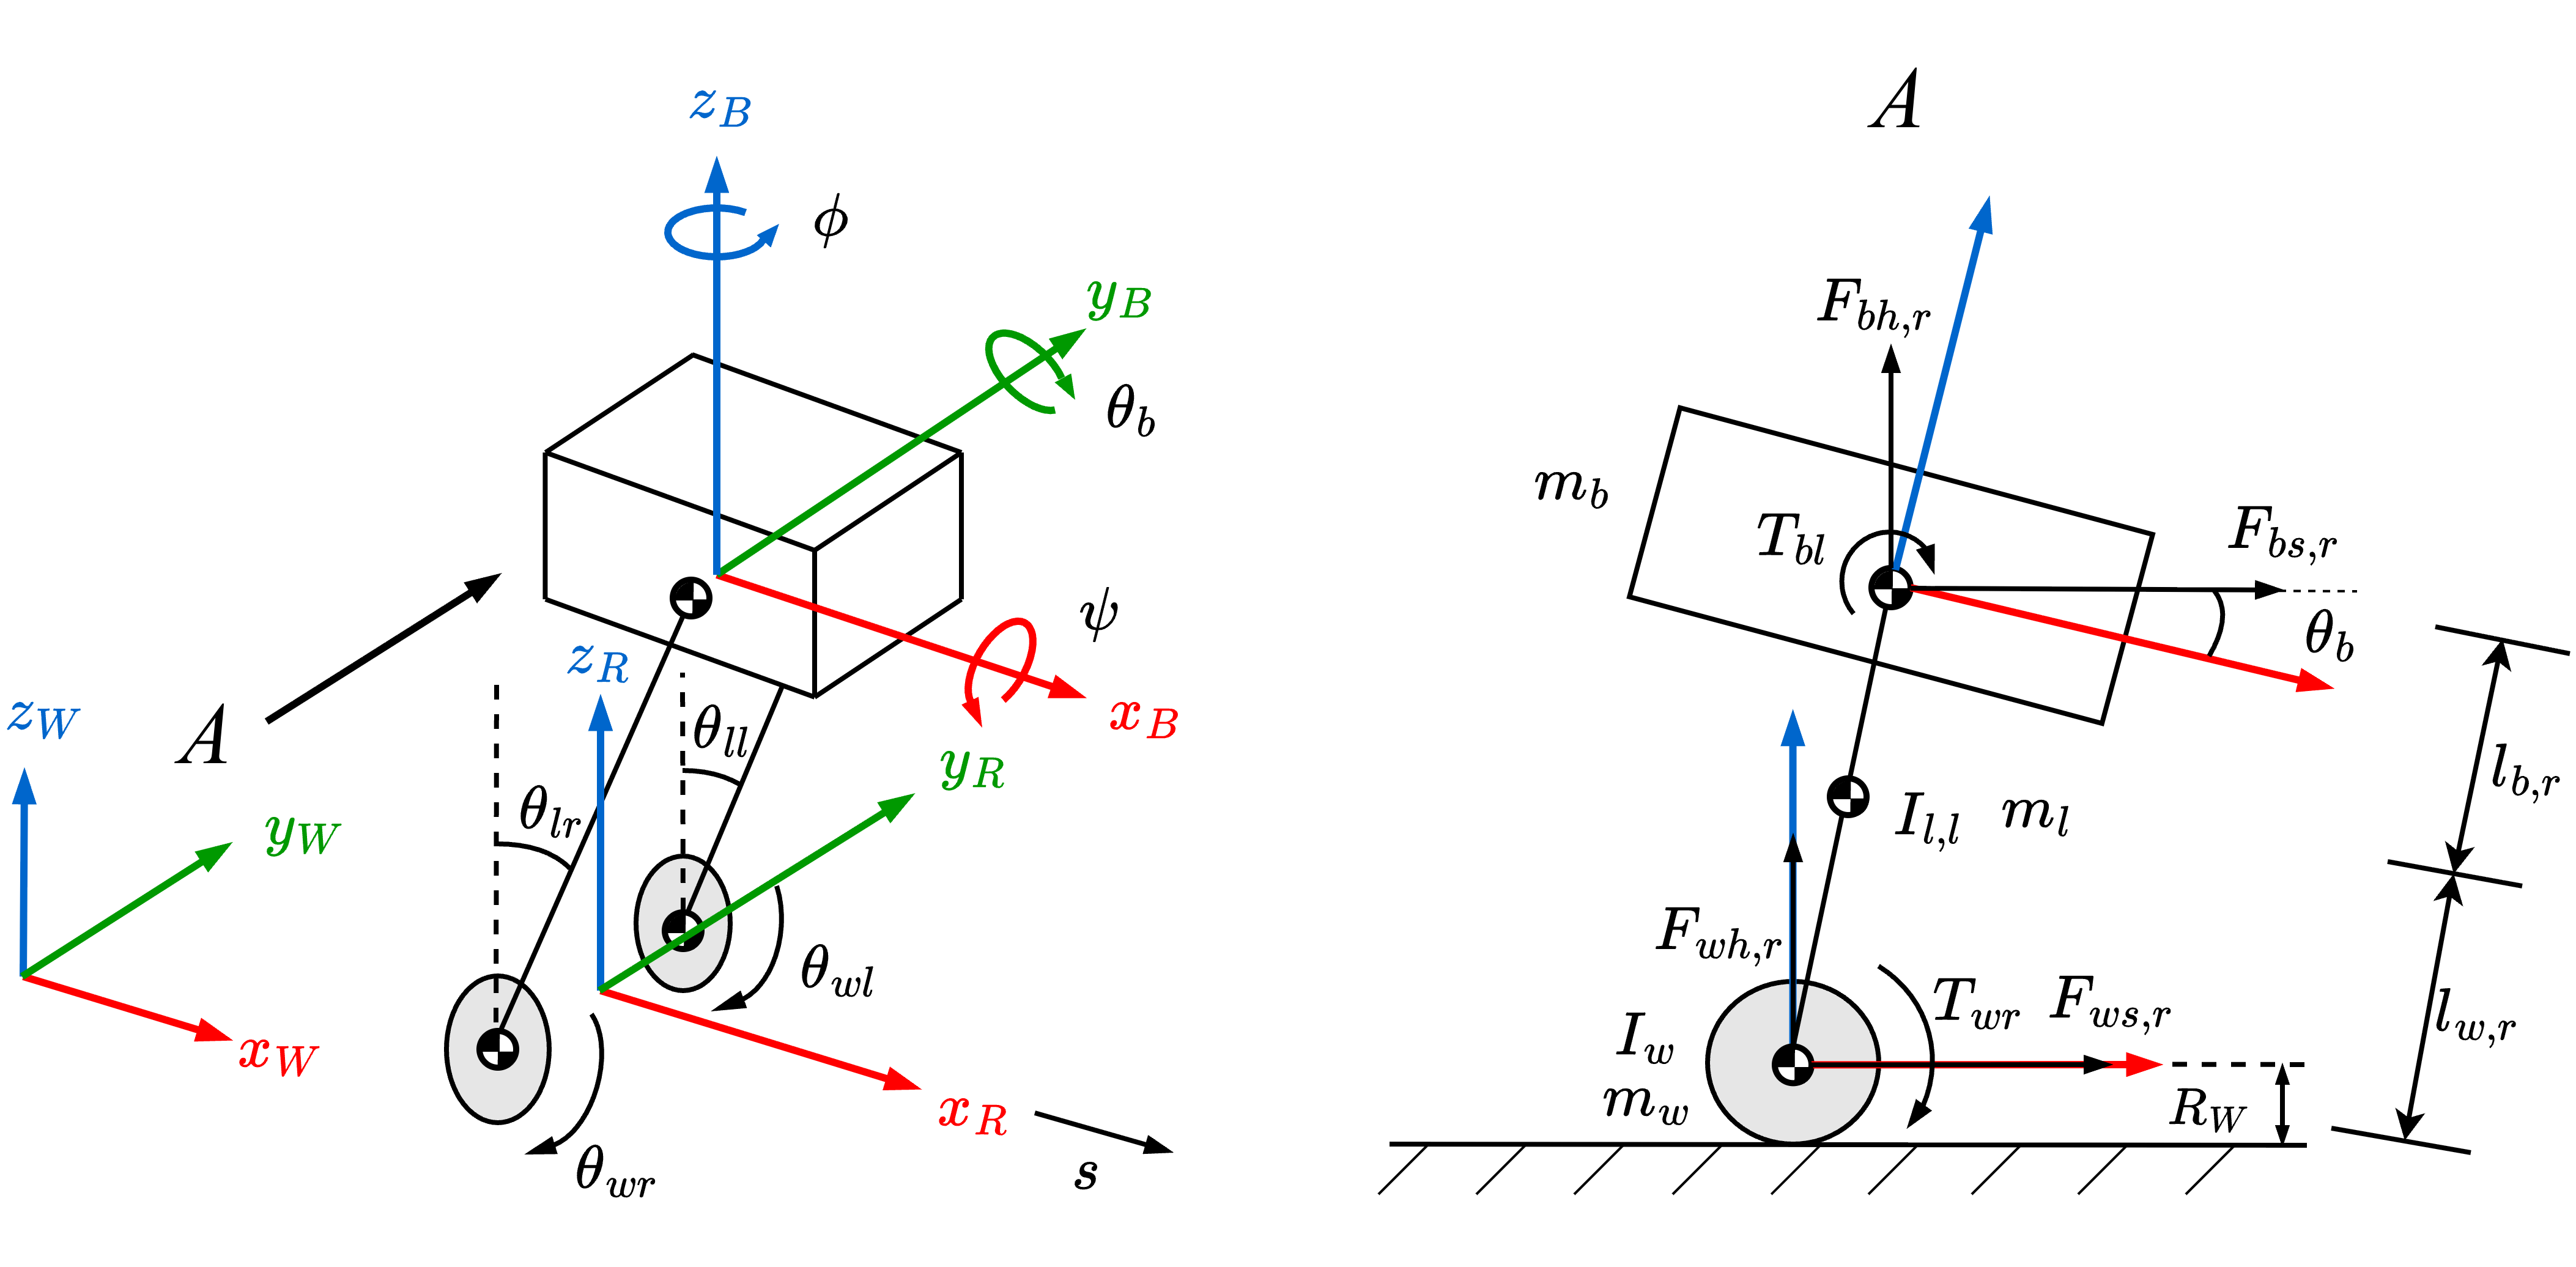
\includegraphics[width=0.88\textwidth]{figures/ch03/wbr_coordinate.png}
  \caption{机器人平面等效模型及坐标系定义}
  \label{fig:model-coordinate}
\end{figure}

为保持全文符号体系统一，将本文涉及的主要符号列于\tabref{tab:model-symbols}。

\begin{table}[htbp]
  \centering
  \caption{模型主要符号定义}\label{tab:model-symbols}
  \renewcommand{\arraystretch}{1.25}
  \begin{tabular}{@{}clp{8.2cm}@{}}
    \toprule
    符号 & 单位 & 含义 \\
    \midrule
    $\theta_{wl}, \theta_{wr}$ & rad & 左、右轮转角 \\
    $\theta_{ll}, \theta_{lr}$ & rad & 左、右虚拟腿摆角 \\
    $\theta_b$ & rad & 机体俯仰角 \\
    $s$ & m & 轮轴中心在惯性坐标系中的水平位移 \\
    $\phi$ & rad & 机器人偏航角，由左右轮差动及腿部横摆共同决定 \\
    $R_w$ & m & 驱动轮半径 \\
    $R_l$ & m & 半轮距，即机器人纵向中面到单侧轮接地点的距离 \\
    $l$ & m & 对称平面建模下的等效虚拟腿长度 \\
    $l_l, l_r$ & m & 左、右腿在偏航近似建模中的等效长度参数；对称工况下可取对应腿长 \\
    $\theta_l$ & rad & 对称平面建模下的平均虚拟腿摆角，满足 $\theta_l=(\theta_{ll}+\theta_{lr})/2$ \\
    $l_b$ & m & 髋关节至机体质心的距离 \\
    $m_w, m_l, m_b$ & kg & 分别表示轮组、虚拟腿等效构件和机体的质量 \\
    $J_w, J_l, J_b$ & kg$\cdot$m$^2$ & 分别表示轮组、虚拟腿等效构件和机体绕质心的转动惯量 \\
    $F_l$ & N & 沿虚拟腿方向的轴向虚拟力 \\
    $T_\theta$ & N$\cdot$m & 绕髋关节作用于虚拟腿的摆动虚拟转矩 \\
    $T_{lw,l}, T_{lw,r}$ & N$\cdot$m & 左、右轮电机输出转矩 \\
    $T_{bl,l}, T_{bl,r}$ & N$\cdot$m & 左、右腿驱动关节输出转矩 \\
    $\boldsymbol{q}$ & -- & 原始广义坐标向量，取 $\boldsymbol{q} = [\theta_{wl},\, \theta_{wr},\, \theta_{ll},\, \theta_{lr},\, \theta_b]^\mathsf{T}$ \\
    $\boldsymbol{q}_v$ & -- & 平面等效模型广义坐标向量，取 $\boldsymbol{q}_v = [s,\, l,\, \theta_l,\, \theta_b]^\mathsf{T}$ \\
    \bottomrule
  \end{tabular}
\end{table}

\subsection{关键点位置关系}

在\figref{fig:model-coordinate} 所示平面模型下，可得轮轴中心、虚拟腿等效质心、髋关节和机体质心在惯性坐标系中的位置分别为
\begin{equation}
  \boldsymbol{p}_W =
  \begin{bmatrix}
    s \\
    R_w
  \end{bmatrix},
  \label{eq:w-pos}
\end{equation}
\begin{equation}
  \boldsymbol{p}_L =
  \begin{bmatrix}
    s + \dfrac{l}{2}\sin\theta_l \\
    R_w + \dfrac{l}{2}\cos\theta_l
  \end{bmatrix},
  \label{eq:l-pos}
\end{equation}
\begin{equation}
  \boldsymbol{p}_H =
  \begin{bmatrix}
    s + l\sin\theta_l \\
    R_w + l\cos\theta_l
  \end{bmatrix},
  \label{eq:h-pos}
\end{equation}
\begin{equation}
  \boldsymbol{p}_B =
  \begin{bmatrix}
    s + l\sin\theta_l + l_b\sin\theta_b \\
    R_w + l\cos\theta_l + l_b\cos\theta_b
  \end{bmatrix}.
  \label{eq:b-pos}
\end{equation}
式中，$\boldsymbol{p}_L$ 用于描述虚拟腿等效构件质心位置，$\boldsymbol{p}_H$ 用于描述髋关节位置，$\boldsymbol{p}_B$ 用于描述机体质心位置。

另一方面，由左右轮纯滚动约束可得
\begin{equation}
  s = \frac{R_w}{2}\left(\theta_{wl} + \theta_{wr}\right),\qquad
  \dot{s} = \frac{R_w}{2}\left(\dot{\theta}_{wl} + \dot{\theta}_{wr}\right),\qquad
  \ddot{s} = \frac{R_w}{2}\left(\ddot{\theta}_{wl} + \ddot{\theta}_{wr}\right).
  \label{eq:rolling-constraint}
\end{equation}
式 \eqref{eq:rolling-constraint} 建立了轮系转角与整机前进位移之间的几何联系，也是后续将轮角变量映射为控制器状态量的基础。对于偏航运动，由于其并非平面模型中的独立广义坐标，相关表达将在第 \ref{sec:state-space-model} 节以运动学映射的形式引入。

\subsection{速度与雅可比关系}

对式 \eqref{eq:l-pos} 和式 \eqref{eq:b-pos} 分别对时间求导，可得虚拟腿等效质心和机体质心的速度表达式
\begin{equation}
  \dot{\boldsymbol{p}}_L =
  \begin{bmatrix}
    \dot{s} + \dfrac{\dot{l}}{2}\sin\theta_l + \dfrac{l\dot{\theta}_l}{2}\cos\theta_l \\
    \dfrac{\dot{l}}{2}\cos\theta_l - \dfrac{l\dot{\theta}_l}{2}\sin\theta_l
  \end{bmatrix},
  \label{eq:l-vel}
\end{equation}
\begin{equation}
  \dot{\boldsymbol{p}}_B =
  \begin{bmatrix}
    \dot{s} + \dot{l}\sin\theta_l + l\dot{\theta}_l\cos\theta_l + l_b\dot{\theta}_b\cos\theta_b \\
    \dot{l}\cos\theta_l - l\dot{\theta}_l\sin\theta_l - l_b\dot{\theta}_b\sin\theta_b
  \end{bmatrix}.
  \label{eq:b-vel}
\end{equation}

将式 \eqref{eq:b-pos} 写成关于等效广义坐标 $\boldsymbol{q}_v$ 的函数形式 $\boldsymbol{p}_B = \boldsymbol{p}_B(\boldsymbol{q}_v)$，则机体质心速度可进一步表示为
\begin{equation}
  \dot{\boldsymbol{p}}_B = \boldsymbol{J}_B(\boldsymbol{q}_v)\dot{\boldsymbol{q}}_v,
  \label{eq:body-jacobian}
\end{equation}
其中，
\begin{equation}
  \boldsymbol{J}_B(\boldsymbol{q}_v) =
  \begin{bmatrix}
    1 & \sin\theta_l & l\cos\theta_l & l_b\cos\theta_b \\
    0 & \cos\theta_l & -l\sin\theta_l & -l_b\sin\theta_b
  \end{bmatrix}.
  \label{eq:body-jacobian-matrix}
\end{equation}

由式 \eqref{eq:l-vel} 至式 \eqref{eq:body-jacobian-matrix} 可见，虚拟腿长度 $l$ 与平均腿摆角 $\theta_l$ 不仅决定整机的几何构型，还通过雅可比矩阵影响机体平动与俯仰运动之间的耦合强度。这一结果说明，采用虚拟腿任务空间描述能够较自然地揭示支撑、摆动与整机姿态之间的运动学联系，为后文动力学建模与任务空间控制设计提供直接依据。

\section{机器人动力学模型}

\subsection{系统能量表达式}

将机器人平面等效模型视为由轮组、虚拟腿等效构件和机体三部分组成，则系统总动能可写为
\begin{equation}
  T = T_w + T_l + T_b,
  \label{eq:kinetic-total}
\end{equation}
其中
\begin{equation}
  T_w = \frac{1}{2}m_w\dot{s}^2 + \frac{1}{2}J_w\left(\frac{\dot{s}}{R_w}\right)^2,
  \label{eq:kinetic-wheel}
\end{equation}
\begin{equation}
  T_l = \frac{1}{2}m_l \dot{\boldsymbol{p}}_L^\mathsf{T}\dot{\boldsymbol{p}}_L + \frac{1}{2}J_l\dot{\theta}_l^2,
  \label{eq:kinetic-leg}
\end{equation}
\begin{equation}
  T_b = \frac{1}{2}m_b \dot{\boldsymbol{p}}_B^\mathsf{T}\dot{\boldsymbol{p}}_B + \frac{1}{2}J_b\dot{\theta}_b^2.
  \label{eq:kinetic-body}
\end{equation}

取地面为势能零位，则系统总势能为
\begin{equation}
  V = m_l g\left(R_w + \frac{l}{2}\cos\theta_l\right) + m_b g\left(R_w + l\cos\theta_l + l_b\cos\theta_b\right),
  \label{eq:potential-total}
\end{equation}
式中，轮组重力势能为常数项，对动力学方程无影响，因此未单独列出。

\subsection{拉格朗日方程与平面等效动力学}

引入平面等效广义坐标
\begin{equation}
  \boldsymbol{q}_v =
  \begin{bmatrix}
    s & l & \theta_l & \theta_b
  \end{bmatrix}^{\mathsf{T}},
  \label{eq:generalized-coordinate-v}
\end{equation}
并定义拉格朗日函数
\begin{equation}
  \mathcal{L} = T - V.
  \label{eq:lagrangian}
\end{equation}
则系统满足
\begin{equation}
  \frac{\mathrm{d}}{\mathrm{d}t}\left(\frac{\partial \mathcal{L}}{\partial \dot{\boldsymbol{q}}_v}\right)
  -
  \frac{\partial \mathcal{L}}{\partial \boldsymbol{q}_v}
  = \boldsymbol{Q}_v,
  \label{eq:lagrange-equation}
\end{equation}
其中广义力向量取为
\begin{equation}
  \boldsymbol{Q}_v =
  \begin{bmatrix}
    \dfrac{T_{lw,l} + T_{lw,r}}{2R_w} \\
    F_l \\
    T_\theta \\
    0
  \end{bmatrix}.
  \label{eq:generalized-force}
\end{equation}
式中，第一个分量表示左右轮驱动转矩在前进方向上的等效广义力，第二、三项分别对应 VMC 作用下的虚拟腿轴向力与摆动虚拟转矩，机体俯仰自由度本身不直接受驱动，故第四项为零。

将式 \eqref{eq:kinetic-total} 至式 \eqref{eq:generalized-force} 代入式 \eqref{eq:lagrange-equation}，可得机器人平面等效模型的动力学方程
\begin{equation}
  \boldsymbol{M}_v(\boldsymbol{q}_v)\ddot{\boldsymbol{q}}_v
  +
  \boldsymbol{C}_v(\boldsymbol{q}_v, \dot{\boldsymbol{q}}_v)\dot{\boldsymbol{q}}_v
  +
  \boldsymbol{G}_v(\boldsymbol{q}_v)
  =
  \boldsymbol{B}_v\boldsymbol{u}_v,
  \label{eq:dynamics-compact}
\end{equation}
其中，
\begin{equation}
  \boldsymbol{u}_v =
  \begin{bmatrix}
    \dfrac{T_{lw,l} + T_{lw,r}}{2} & F_l & T_\theta
  \end{bmatrix}^{\mathsf{T}},\qquad
  \boldsymbol{B}_v =
  \begin{bmatrix}
    1/R_w & 0 & 0 \\
    0 & 1 & 0 \\
    0 & 0 & 1 \\
    0 & 0 & 0
  \end{bmatrix}.
  \label{eq:input-matrix}
\end{equation}

系统质量矩阵 $\boldsymbol{M}_v(\boldsymbol{q}_v)$ 具体为
\begin{equation}
  \boldsymbol{M}_v(\boldsymbol{q}_v) =
  \begin{bmatrix}
    m_w + m_l + m_b + J_w/R_w^2 &
    \left(\dfrac{m_l}{2} + m_b\right)\sin\theta_l &
    \left(\dfrac{m_l}{2} + m_b\right)l\cos\theta_l &
    m_b l_b \cos\theta_b \\
    \left(\dfrac{m_l}{2} + m_b\right)\sin\theta_l &
    \dfrac{m_l}{4} + m_b &
    0 &
    m_b l_b \sin(\theta_l - \theta_b) \\
    \left(\dfrac{m_l}{2} + m_b\right)l\cos\theta_l &
    0 &
    J_l + \dfrac{m_l l^2}{4} + m_b l^2 &
    m_b l l_b \cos(\theta_l - \theta_b) \\
    m_b l_b \cos\theta_b &
    m_b l_b \sin(\theta_l - \theta_b) &
    m_b l l_b \cos(\theta_l - \theta_b) &
    J_b + m_b l_b^2
  \end{bmatrix},
  \label{eq:mass-matrix}
\end{equation}
重力项向量为
\begin{equation}
  \boldsymbol{G}_v(\boldsymbol{q}_v) =
  \begin{bmatrix}
    0 \\
    \left(\dfrac{m_l}{2} + m_b\right) g\cos\theta_l \\
    -\left(\dfrac{m_l}{2} + m_b\right) gl\sin\theta_l \\
    -m_b g l_b \sin\theta_b
  \end{bmatrix}.
  \label{eq:gravity-vector}
\end{equation}
科氏力项和离心力项由矩阵 $\boldsymbol{C}_v(\boldsymbol{q}_v, \dot{\boldsymbol{q}}_v)$ 描述，其元素可由 Christoffel 符号统一构造：
\begin{equation}
  C_{ij} = \frac{1}{2}\sum_{k=1}^{4}
  \left(
    \frac{\partial M_{ij}}{\partial q_k}
    +
    \frac{\partial M_{ik}}{\partial q_j}
    -
    \frac{\partial M_{jk}}{\partial q_i}
  \right)\dot{q}_k.
  \label{eq:christoffel}
\end{equation}

式 \eqref{eq:dynamics-compact} 表明，平面等效模型已经显式体现出前进位移、腿长、腿摆和机体俯仰之间的耦合关系。特别地，$l$ 的变化会同时影响惯性分布与重力项，而 $\theta_l$ 的变化则通过三角函数项改变整机俯仰耦合强度。与直接在关节空间独立处理各驱动量相比，基于平面等效模型开展控制设计更容易保留这些物理耦合关系，这也是本文后续采用分层控制结构的重要建模依据。

\section{面向控制设计的线性化状态空间模型}\label{sec:state-space-model}

前述平面等效模型主要服务于对整机力学关系的理解与任务空间控制量的构造。为了与第四章的 LQR 设计相衔接，本节进一步回到原始五自由度独立广义坐标模型，补充从广义动力学方程到标准线性状态空间模型的推导过程。

\subsection{独立广义坐标与广义动力学线性化}

以式 \eqref{eq:generalized-coordinate-origin} 所示五个独立广义坐标和式 \eqref{eq:input-origin} 所示四个输入力矩为基础，可通过牛顿--欧拉法或拉格朗日法建立机器人原始动力学方程。该过程中需要同时处理轮组、左右腿和机体之间的约束力。经过约束消元后，可将系统写成仅含独立广义坐标的二阶动力学形式。对于直立平衡点附近的小角度运动，进一步忽略高阶非线性项，可得线性化后的广义动力学方程
\begin{equation}
  \boldsymbol{M}\ddot{\boldsymbol{q}} + \boldsymbol{K}\boldsymbol{q} = \boldsymbol{E}\boldsymbol{u},
  \label{eq:linearized-generalized-model-ch3}
\end{equation}
其中，$\boldsymbol{M}$ 为平衡点处的等效惯性矩阵，$\boldsymbol{K}$ 为线性化后由重力项和耦合项构成的刚度矩阵，$\boldsymbol{E}$ 为输入分配矩阵。由于 $\boldsymbol{M}$ 在工作点附近非奇异，故式 \eqref{eq:linearized-generalized-model-ch3} 可进一步改写为
\begin{equation}
  \ddot{\boldsymbol{q}}
  =
  \boldsymbol{A}_{\mathrm{dyn}}\boldsymbol{q}
  +
  \boldsymbol{B}_{\mathrm{dyn}}\boldsymbol{u},
  \qquad
  \boldsymbol{A}_{\mathrm{dyn}} = -\boldsymbol{M}^{-1}\boldsymbol{K},
  \qquad
  \boldsymbol{B}_{\mathrm{dyn}} = \boldsymbol{M}^{-1}\boldsymbol{E}.
  \label{eq:qdd-dyn-ch3}
\end{equation}

式 \eqref{eq:qdd-dyn-ch3} 给出了广义坐标空间中的加速度表达式，但第四章的控制器并不直接以轮角为状态，而是采用更具物理意义的前进位移、偏航角、左右腿摆角和机体俯仰角构造状态向量。因此，还需进一步建立从广义坐标到控制器状态量的运动学映射关系。

\subsection{状态向量定义与运动学映射}

为突出机器人在平衡与转向过程中的实际运动状态，定义位置状态向量与完整状态向量分别为
\begin{equation}
  \boldsymbol{x}_{\mathrm{pos}}
  =
  \begin{bmatrix}
    s & \phi & \theta_{ll} & \theta_{lr} & \theta_b
  \end{bmatrix}^{\mathsf{T}},
  \label{eq:xpos-ch3}
\end{equation}
\begin{equation}
  \boldsymbol{x}
  =
  \begin{bmatrix}
    s & \dot{s} & \phi & \dot{\phi} & \theta_{ll} & \dot{\theta}_{ll} &
    \theta_{lr} & \dot{\theta}_{lr} & \theta_b & \dot{\theta}_b
  \end{bmatrix}^{\mathsf{T}}.
  \label{eq:state-vector-ch3}
\end{equation}
其中，前进位移 $s$ 已由式 \eqref{eq:rolling-constraint} 给出。偏航角 $\phi$ 虽不是原始模型中的独立广义坐标，但可由左右轮差动和左右腿摆动的几何关系近似表示为
\begin{equation}
  \phi
  =
  \frac{R_w}{2R_l}\left(-\theta_{wl} + \theta_{wr}\right)
  -
  \frac{l_l}{2R_l}\sin \theta_{ll}
  +
  \frac{l_r}{2R_l}\sin \theta_{lr}.
  \label{eq:yaw-kinematic-map-ch3}
\end{equation}
式 \eqref{eq:yaw-kinematic-map-ch3} 说明，偏航姿态不仅受轮差动驱动影响，也与左右腿摆角变化有关。对式 \eqref{eq:yaw-kinematic-map-ch3} 在直立平衡点附近作小角度线性化，并忽略 $\dot{\theta}^2$ 等高阶项，可得
\begin{equation}
  \ddot{\phi}
  \approx
  \frac{R_w}{2R_l}\left(-\ddot{\theta}_{wl} + \ddot{\theta}_{wr}\right)
  -
  \frac{l_l}{2R_l}\ddot{\theta}_{ll}
  +
  \frac{l_r}{2R_l}\ddot{\theta}_{lr}.
  \label{eq:yaw-acc-linear-ch3}
\end{equation}

进一步定义状态加速度向量
\begin{equation}
  \boldsymbol{x}_{\mathrm{acc}}
  =
  \begin{bmatrix}
    \ddot{s} & \ddot{\phi} & \ddot{\theta}_{ll} & \ddot{\theta}_{lr} & \ddot{\theta}_b
  \end{bmatrix}^{\mathsf{T}},
  \label{eq:xacc-ch3}
\end{equation}
则由式 \eqref{eq:rolling-constraint} 和式 \eqref{eq:yaw-acc-linear-ch3} 可得，$\boldsymbol{x}_{\mathrm{acc}}$ 与广义加速度 $\ddot{\boldsymbol{q}}$ 之间满足线性映射
\begin{equation}
  \boldsymbol{x}_{\mathrm{acc}} = \boldsymbol{T}_{\mathrm{map}}\ddot{\boldsymbol{q}},
  \label{eq:tmap-def-ch3}
\end{equation}
其中，
\begin{equation}
  \boldsymbol{T}_{\mathrm{map}}
  =
  \begin{bmatrix}
    \dfrac{R_w}{2} & \dfrac{R_w}{2} & 0 & 0 & 0 \\
    -\dfrac{R_w}{2R_l} & \dfrac{R_w}{2R_l} & -\dfrac{l_l}{2R_l} & \dfrac{l_r}{2R_l} & 0 \\
    0 & 0 & 1 & 0 & 0 \\
    0 & 0 & 0 & 1 & 0 \\
    0 & 0 & 0 & 0 & 1
  \end{bmatrix}.
  \label{eq:tmap-ch3}
\end{equation}

另一方面，在小角度线性化条件下，式 \eqref{eq:rolling-constraint} 和式 \eqref{eq:yaw-kinematic-map-ch3} 还可用于将原始广义坐标表示为位置状态的线性组合，即
\begin{equation}
  \boldsymbol{q}
  =
  \boldsymbol{P}\boldsymbol{x}_{\mathrm{pos}},
  \label{eq:q-xpos-map-def-ch3}
\end{equation}
其中，
\begin{equation}
  \boldsymbol{P}
  =
  \begin{bmatrix}
    \dfrac{1}{R_w} & -\dfrac{R_l}{R_w} & -\dfrac{l_l}{2R_w} & \dfrac{l_r}{2R_w} & 0 \\
    \dfrac{1}{R_w} & \dfrac{R_l}{R_w} & \dfrac{l_l}{2R_w} & -\dfrac{l_r}{2R_w} & 0 \\
    0 & 0 & 1 & 0 & 0 \\
    0 & 0 & 0 & 1 & 0 \\
    0 & 0 & 0 & 0 & 1
  \end{bmatrix}.
  \label{eq:q-xpos-map-ch3}
\end{equation}
式 \eqref{eq:tmap-ch3} 与式 \eqref{eq:q-xpos-map-ch3} 分别给出了“广义加速度到状态加速度”和“位置状态到广义坐标”的桥接关系，从而为建立标准状态空间表达式提供了中间映射。

\subsection{线性状态空间方程建立}

将状态向量式 \eqref{eq:state-vector-ch3} 按位置与速度两部分分解，可写为
\begin{equation}
  \boldsymbol{x}
  =
  \begin{bmatrix}
    \boldsymbol{x}_{\mathrm{pos}} \\
    \dot{\boldsymbol{x}}_{\mathrm{pos}}
  \end{bmatrix},
  \qquad
  \dot{\boldsymbol{x}}
  =
  \begin{bmatrix}
    \dot{\boldsymbol{x}}_{\mathrm{pos}} \\
    \boldsymbol{x}_{\mathrm{acc}}
  \end{bmatrix}.
  \label{eq:x-split-ch3}
\end{equation}
将式 \eqref{eq:qdd-dyn-ch3}、式 \eqref{eq:tmap-def-ch3} 与式 \eqref{eq:q-xpos-map-def-ch3} 依次联立，可得
\begin{equation}
  \boldsymbol{x}_{\mathrm{acc}}
  =
  \boldsymbol{T}_{\mathrm{map}}
  \left(
    \boldsymbol{A}_{\mathrm{dyn}}\boldsymbol{q}
    +
    \boldsymbol{B}_{\mathrm{dyn}}\boldsymbol{u}
  \right)
  =
  \boldsymbol{T}_{\mathrm{map}}\boldsymbol{A}_{\mathrm{dyn}}\boldsymbol{P}\boldsymbol{x}_{\mathrm{pos}}
  +
  \boldsymbol{T}_{\mathrm{map}}\boldsymbol{B}_{\mathrm{dyn}}\boldsymbol{u}.
  \label{eq:xacc-from-qdd-ch3}
\end{equation}
记
\begin{equation}
  \boldsymbol{A}_p = \boldsymbol{T}_{\mathrm{map}}\boldsymbol{A}_{\mathrm{dyn}}\boldsymbol{P},
  \qquad
  \boldsymbol{B}_p = \boldsymbol{T}_{\mathrm{map}}\boldsymbol{B}_{\mathrm{dyn}},
  \label{eq:ap-bp-ch3}
\end{equation}
则式 \eqref{eq:x-split-ch3} 可整理为标准连续时间线性状态空间形式
\begin{equation}
  \dot{\boldsymbol{x}}
  =
  \boldsymbol{A}\boldsymbol{x}
  +
  \boldsymbol{B}\boldsymbol{u},
  \label{eq:linear-state-space-ch3}
\end{equation}
其中
\begin{equation}
  \boldsymbol{A}
  =
  \begin{bmatrix}
    \boldsymbol{0}_{5\times5} & \boldsymbol{I}_{5\times5} \\
    \boldsymbol{A}_p & \boldsymbol{0}_{5\times5}
  \end{bmatrix},
  \qquad
  \boldsymbol{B}
  =
  \begin{bmatrix}
    \boldsymbol{0}_{5\times4} \\
    \boldsymbol{B}_p
  \end{bmatrix}.
  \label{eq:ab-matrix-ch3}
\end{equation}

式 \eqref{eq:linear-state-space-ch3} 至式 \eqref{eq:ab-matrix-ch3} 给出了从原始广义动力学方程到控制器所需状态空间模型的完整推导链条。需要指出的是，本文此处的目标并非将 $\boldsymbol{A}$、$\boldsymbol{B}$ 的各元素全部解析展开，而是明确其来源：先在广义坐标空间求得加速度表达式，再通过运动学映射转化为控制器状态变量上的线性模型。这样处理既保留了第三章建模与第四章控制设计之间的逻辑连续性，也避免了在正文中展开冗长而低信息量的矩阵元素计算。

\section{五连杆机构的任务空间映射与 VMC 力矩转换}

前几节给出的整机模型主要服务于平衡控制器设计，而实际样机的单腿仍为五连杆闭环机构。为使虚拟腿空间中的支撑力和摆动转矩能够落实为关节驱动力矩，本节进一步建立主动关节空间与虚拟腿任务空间之间的映射关系。

\subsection{五连杆闭环运动学}

本文腿部机构的几何构型可直接沿用第二章的机构简图（\figref{fig:leg-linkage}）。为与全文记号一致，将两个主动关节角记为 $\theta_{ll}$、$\theta_{lr}$，两个被动关节角记为 $\theta_{pl}$、$\theta_{pr}$，基座两铰点为 $A$、$D$，末端汇交点为 $P$。根据闭环几何约束，有
\begin{equation}
  \boldsymbol{p}_A + l_1 \boldsymbol{e}(\theta_{ll}) + l_2 \boldsymbol{e}(\theta_{pl})
  =
  \boldsymbol{p}_D + l_4 \boldsymbol{e}(\theta_{lr}) + l_3 \boldsymbol{e}(\theta_{pr})
  =
  \boldsymbol{p}_P,
  \label{eq:fivebar-loop}
\end{equation}
其中，
\begin{equation}
  \boldsymbol{e}(q) =
  \begin{bmatrix}
    \cos q \\
    \sin q
  \end{bmatrix}.
  \label{eq:unit-vector}
\end{equation}

由式 \eqref{eq:fivebar-loop} 可解得末端点 $P$ 的位置 $\boldsymbol{p}_P = [p_s,\ p_h]^\mathsf{T}$，进而定义虚拟腿变量
\begin{equation}
  l = \sqrt{p_s^2 + p_h^2},\qquad
  \theta_l = \operatorname{atan2}(p_s,\, p_h).
  \label{eq:virtual-leg-from-fivebar}
\end{equation}
式 \eqref{eq:virtual-leg-from-fivebar} 表明，五连杆机构虽为闭环结构，但其末端几何关系最终仍可等效为虚拟腿长度 $l$ 和平均虚拟腿摆角 $\theta_l$ 两个任务空间变量。对式 \eqref{eq:virtual-leg-from-fivebar} 求导，可得
\begin{equation}
  \begin{bmatrix}
    \dot{l} \\
    \dot{\theta}_l
  \end{bmatrix}
  =
  \begin{bmatrix}
    \dfrac{p_s}{l} & \dfrac{p_h}{l} \\
    \dfrac{p_h}{l^2} & -\dfrac{p_s}{l^2}
  \end{bmatrix}
  \dot{\boldsymbol{p}}_P.
  \label{eq:lp-theta-from-p}
\end{equation}

若将主动关节向量记为
\begin{equation}
  \boldsymbol{q}_a =
  \begin{bmatrix}
    \theta_{ll} & \theta_{lr}
  \end{bmatrix}^{\mathsf{T}},
  \label{eq:active-joint-vector-ch3}
\end{equation}
并记末端点速度雅可比矩阵为 $\boldsymbol{J}_P(\boldsymbol{q}_a)$，则有
\begin{equation}
  \dot{\boldsymbol{p}}_P = \boldsymbol{J}_P(\boldsymbol{q}_a)\dot{\boldsymbol{q}}_a.
  \label{eq:endpoint-jacobian}
\end{equation}
联立式 \eqref{eq:lp-theta-from-p} 和式 \eqref{eq:endpoint-jacobian}，可得虚拟腿空间与主动关节空间之间的速度映射关系
\begin{equation}
  \begin{bmatrix}
    \dot{l} \\
    \dot{\theta}_l
  \end{bmatrix}
  =
  \boldsymbol{J}_v(\boldsymbol{q}_a)\dot{\boldsymbol{q}}_a,
  \qquad
  \boldsymbol{J}_v(\boldsymbol{q}_a) =
  \begin{bmatrix}
    \dfrac{p_s}{l} & \dfrac{p_h}{l} \\
    \dfrac{p_h}{l^2} & -\dfrac{p_s}{l^2}
  \end{bmatrix}
  \boldsymbol{J}_P(\boldsymbol{q}_a).
  \label{eq:virtual-jacobian}
\end{equation}

\subsection{基于 VMC 的关节力矩映射}

VMC 的核心在于先在任务空间中构造期望虚拟力，再利用雅可比矩阵将其映射到关节空间。根据虚功原理，有
\begin{equation}
  \delta W = \boldsymbol{\tau}^\mathsf{T}\delta\boldsymbol{q}_a
  =
  \boldsymbol{F}_v^\mathsf{T}\delta\boldsymbol{x}_v,
  \label{eq:virtual-work}
\end{equation}
其中，
\begin{equation}
  \boldsymbol{\tau} =
  \begin{bmatrix}
    \tau_1 \\
    \tau_2
  \end{bmatrix},
  \qquad
  \boldsymbol{x}_v =
  \begin{bmatrix}
    l \\
    \theta_l
  \end{bmatrix}.
  \label{eq:joint-torque-and-state}
\end{equation}
又由 $\delta\boldsymbol{x}_v = \boldsymbol{J}_v \delta\boldsymbol{q}_a$，可得
\begin{equation}
  \boldsymbol{\tau} = \boldsymbol{J}_v^\mathsf{T}\boldsymbol{F}_v
  =
  \boldsymbol{J}_v^\mathsf{T}
  \begin{bmatrix}
    F_l \\
    T_\theta
  \end{bmatrix}.
  \label{eq:vmc-torque-map}
\end{equation}

式 \eqref{eq:vmc-torque-map} 给出了从虚拟腿任务空间到五连杆主动关节空间的力矩映射关系。对本文腿部机构而言，$F_l$ 主要负责腿长支撑、缓冲与高度调节，$T_\theta$ 主要负责腿部前后摆动及姿态辅助调节。由此，任务空间中的控制目标便能够通过解析映射直接转化为实际执行器的驱动力矩。

\subsection{五连杆动力学表达}

考虑五连杆机构的主动关节空间动力学，可写为
\begin{equation}
  \boldsymbol{M}_5(\boldsymbol{q}_a)\ddot{\boldsymbol{q}}_a
  +
  \boldsymbol{C}_5(\boldsymbol{q}_a, \dot{\boldsymbol{q}}_a)\dot{\boldsymbol{q}}_a
  +
  \boldsymbol{G}_5(\boldsymbol{q}_a)
  =
  \boldsymbol{\tau}
  -
  \boldsymbol{J}_e^\mathsf{T}(\boldsymbol{q}_a)\boldsymbol{F}_{\mathrm{ext}},
  \label{eq:fivebar-dynamics}
\end{equation}
其中，$\boldsymbol{M}_5(\boldsymbol{q}_a)$ 为五连杆主动关节空间惯性矩阵，$\boldsymbol{C}_5(\boldsymbol{q}_a, \dot{\boldsymbol{q}}_a)$ 为科氏力和离心力矩阵，$\boldsymbol{G}_5(\boldsymbol{q}_a)$ 为重力项，$\boldsymbol{J}_e(\boldsymbol{q}_a)$ 为末端接触雅可比矩阵，$\boldsymbol{F}_{\mathrm{ext}}$ 为地面接触力或其他外部载荷。

将式 \eqref{eq:vmc-torque-map} 代入式 \eqref{eq:fivebar-dynamics}，可得五连杆机构在 VMC 作用下的动力学表达式
\begin{equation}
  \boldsymbol{M}_5(\boldsymbol{q}_a)\ddot{\boldsymbol{q}}_a
  +
  \boldsymbol{C}_5(\boldsymbol{q}_a, \dot{\boldsymbol{q}}_a)\dot{\boldsymbol{q}}_a
  +
  \boldsymbol{G}_5(\boldsymbol{q}_a)
  =
  \boldsymbol{J}_v^\mathsf{T}(\boldsymbol{q}_a)\boldsymbol{F}_v
  -
  \boldsymbol{J}_e^\mathsf{T}(\boldsymbol{q}_a)\boldsymbol{F}_{\mathrm{ext}}.
  \label{eq:fivebar-vmc-dynamics}
\end{equation}
式 \eqref{eq:fivebar-vmc-dynamics} 表明，五连杆机构的关节动力学可以统一理解为“虚拟力驱动项”与“外部接触载荷项”的叠加。因而，当给定虚拟腿长度和虚拟腿摆角的目标轨迹后，可先利用式 \eqref{eq:vmc-law} 生成虚拟力 $\boldsymbol{F}_v$，再由式 \eqref{eq:vmc-torque-map} 求得主动关节力矩命令，从而完成从任务空间目标到底层执行器控制量的闭环映射。

\section{本章小结}

本章围绕第四章控制系统设计的需求，完成了双轮足机器人的建模工作。首先，在统一变量和基本假设的基础上，将闭环腿部机构等效为可伸缩虚拟杆，明确了 VMC 中的轴向虚拟力 $F_l$ 与摆动虚拟转矩 $T_\theta$。随后，建立了平面等效模型的坐标系、关键点位置关系与速度雅可比表达，并基于拉格朗日方法推导出整机动力学方程及相应的质量矩阵、重力项和输入矩阵。在此基础上，进一步补充了从原始广义动力学方程到线性状态空间方程的推导，说明了控制器状态向量、广义坐标与运动学映射之间的关系。最后，针对实际五连杆机构给出了闭环运动学、虚拟腿雅可比矩阵以及任务空间到关节空间的力矩映射，从而将“整机动力学建模”“状态空间控制模型”和“腿部任务空间执行模型”贯通起来，为第四章分层控制器设计提供了统一模型基础。
